\chapter{Updating the Swift runtime}
\label{ch:UpdatingRuntime}

\section{Introduction}
\label{sec:Introduction}

In this chapter, we delve into the process of updating the Swift Runtime for OpenWhisk, a critical component of our exploration of Swift as a serverless language. One of the key elements of this exploration is the transition from Swift 5.4 to Swift 5.8. This version update brings with it a wealth of new features that greatly enhance the capabilities of Swift as a serverless language, including concurrency support (via async/await constructs), structured concurrency, the actor model, and SwiftNIO 2.

These features provide significant benefits when it comes to the development and deployment of serverless applications. In particular, they have a profound impact on our synchronization system case study. For instance, the async/await constructs, part of the concurrency support, simplify the handling of asynchronous tasks, making the code easier to write and understand. This was particularly beneficial in the development of both a monolithic and a serverless implementation of the synchronization system, which heavily relied on these constructs.

Runtimes in OpenWhisk are the backbone that enables the execution of actions in the serverless environment. Key to this is understanding the Action Interface and the ActionLoop Proxy. The ActionLoop proxy simplifies the development of new runtimes by implementing most of the Action Interface specification, making it possible to create a compliant and efficient runtime with fewer resources.

Updating the Swift runtime in itself was not complicated, but understanding how it all works together was a challenge. In this chapter we dive into the details of how this is achieved, to provide a reference point for future researches in understanding how OpenWhisk runtimes work, and particularly the Swift runtime.

\section{Swift 5.5 Enhancements and their Impact}
\label{sec:SwiftEnhancements}

We elucidate how these enhancements facilitated the development and benchmarking of a monolithic and a serverless implementation in the synchronization system case study, with a focus on the substantial use of the async/await constructs in the pre-existing monolithic implementation.
\subsection{Concurrency Support and Async/Await}
\label{subsec:ConcurrencySupport}

In Swift 5.5, the introduction of concurrency support, in particular, the async/await constructs, revolutionized the way asynchronous code is written and understood. The async/await model allows for the execution of asynchronous tasks in a manner that closely resembles synchronous code, eliminating the complexity of nested callbacks and error-prone manual threading.

In the context of our synchronization system case study, this feature had a profound impact. The pre-existing monolithic implementation was built with heavy use of asynchronous constructs. With the transition to Swift 5.5, we could leverage the async/await model to handle these tasks in a more readable and maintainable way, making the code easier to comprehend and modify.

\subsection{Structured Concurrency}
\label{subsec:StructuredConcurrency}

Structured concurrency, another significant feature introduced in Swift 5.5, provides a way to manage and control asynchronous tasks. It introduces new concepts like task groups and task cancellation, which can be used to group related tasks and cancel them if they are no longer needed.

For the synchronization system case study, structured concurrency helped ensure that asynchronous tasks were well-managed and tidied up after completion. This reduced the risk of memory leaks and made the system more efficient.

\subsection{Actor Model}
\label{subsec:ActorModel}

The actor model in Swift 5.5 provides a way to handle shared mutable state in concurrent settings. It isolates state to individual actors and ensures that only one piece of code can access that state at a time.

In the context of the synchronization system, the actor model was invaluable in managing shared resources, avoiding race conditions and thus increasing the robustness of the system.

\subsection{SwiftNIO 2}
\label{subsec:SwiftNIO}

SwiftNIO 2, a low-level tool for building high-performance networking applications, brought about enhancements that improved the performance and functionality of our serverless implementation. It enabled the efficient handling of networking tasks in the synchronization system, resulting in a performance boost and more robust networking capabilities.

\subsection{Impact on the Synchronization System Case Study}
\label{subsec:ImpactCaseStudy}

Overall, the enhancements in Swift 5.5 significantly improved the development and benchmarking process for both the monolithic and serverless implementations of the synchronization system. The async/await constructs, structured concurrency, the actor model, and SwiftNIO 2 all contributed to a more efficient, maintainable, and robust system. They allowed us to write cleaner, more understandable code, manage asynchronous tasks more effectively, avoid common concurrency issues, and handle networking tasks more efficiently. This demonstrated the potential of Swift 5.5 as a powerful language for serverless computing.

\section{Understanding Runtimes in OpenWhisk}
\label{sec:OpenWhiskRuntimes}

We delve into the function and significance of runtimes in OpenWhisk, paying special attention to the role of the ActionLoop proxy and Action Interface. We clarify how the ActionLoop proxy aids in the creation of compliant runtimes by implementing most of the specification, enabling the development of an efficient runtime in a short span of time.
\section{Actions in OpenWhisk}

\subsection{Action Interface in OpenWhisk}
The core concept in the OpenWhisk environment is an Action. Actions are the smallest deployable units of code and primarily constitute two components: the user function and its corresponding proxy. The user function represents the code logic to be executed, and the proxy serves as an intermediary, implementing a canonical protocol to enable the user function to interact with the OpenWhisk platform \cite{action-interface}. The proxy is the runtime. Anything can be a runtime, as far as OpenWhisk is concerned, as long as it implments the Action Interface, which specifies a behavior that OpenWhisk expects. In other words, a runtime can be thought of a black box (docker container) that listens on two HTTP routes: /init and /run on port 8080, which are used for deploying and executing actions, respectively. OpenWhisk calls on the /init route with the action code to initialize an action. Whenever the action is invoked, OpenWhisk will send a POST request  to the /run route with the action's parameters as payload. The runtime should return the result of the action. The behavior is shown abstractly in figure 2.1.
\begin{figure}[h]
    \centering
    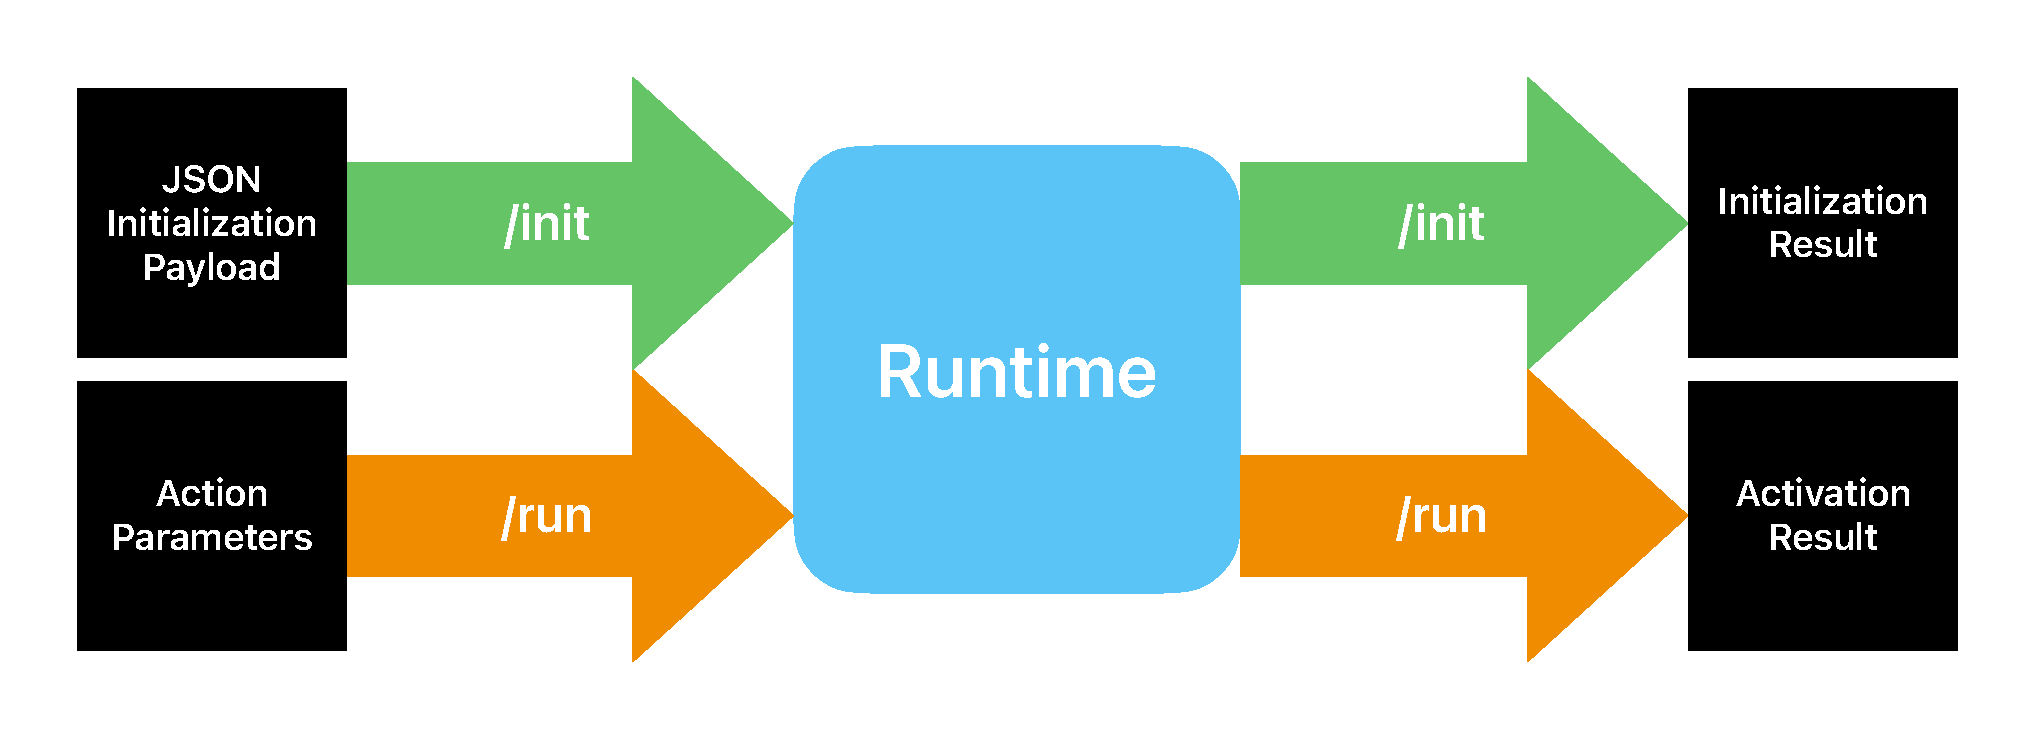
\includegraphics[width=\textwidth]{media/action_interface.pdf}
    \caption{Abstract representation of the Action Interface in OpenWhisk.}
    \label{fig:actioninterface}
\end{figure}

The /init endpoint is tasked with container initialization and accepts a POST request consisting of a JSON object that includes the action name, function to be executed, the source code, and several environment variables. This initialization happens exactly once and must be completed within a predefined time limit set by the platform \cite{action-interface}.

Once initialization is completed successfully, the runtime transitions to a state where it can activate the function. The /run endpoint is responsible for this task. It receives an HTTP POST request with a new activation context and the function's input parameters. The route needs to accept a JSON object and respond with one, adhering to the OpenWhisk platform's prescribed schema. Every action in OpenWhisk has a set time limit, within which the activation must complete. If the function executes successfully, the route responds with 200 OK, and the response body is recorded as the result of the activation \cite{openwhisk2023}.

The runtime should flush all the logs generated during initialization and execution, adding a unique frame marker at the end of each activation log stream. This marker is necessary to avoid delayed or truncated activation logs \cite{openwhisk2023}.

\subsection{ActionLoop Proxy in OpenWhisk}

The ActionLoop proxy is a tool designed to simplify the process of creating new OpenWhisk runtimes. While one can develop a new runtime by following the Action Interface, the ActionLoop proxy offers a quicker and more efficient way to achieve this by implementing most of the specification out-of-the-box \cite{action-proxy}.

The ActionLoop proxy is a runtime engine, developed in Go, initially designed to support the OpenWhisk Go language runtime. However, its generic design allows it to be adapted for other language runtimes such as Swift, PHP, Python, Rust, Java, Ruby, and Crystal. It was engineered keeping both compiled and scripting languages in mind.

Using the ActionLoop proxy, one can develop a new runtime in a fraction of the time it would take to create one from scratch. This is due to the fact that the ActionLoop proxy requires the developer to write only a command line protocol instead of a full-fledged web server, reducing complexity. Additionally, the ActionLoop proxy is known to significantly enhance the performance of existing runtimes, providing speed improvements ranging from 2x to 20x \cite{action-proxy}.

Since Swift, like all other language runtimes except Javascript, leverage it, understanding the ActioxnLoop proxy is crucial to be able to update the OpenWhisk runtime to support the latest version of Swift, enhancing the potential for Swift to be used as a Serverless language.

\subsection{Compiling a Swift action with the ActionLoop Proxy}

\section{Overview of the officially supported Swift runtime in OpenWhisk}
Apache OpenWhisk supports a variety of programming languages for writing actions, through the use of specific runtimes. As per the official documentation, the following runtimes are currently supported 
~\cite{openwhisk2023}:

\begin{itemize}
\item .Net: OpenWhisk runtime for .Net Core 2.2.
\item Go: OpenWhisk runtime for Go.
\item Java: OpenWhisk runtime for Java 8 (OpenJDK 8, JVM OpenJ9).
\item JavaScript: OpenWhisk runtime for Node.js v10, v12, and v14.
\item PHP: OpenWhisk runtime for PHP 8.0, 7.4, and 7.3.
\item Python: OpenWhisk runtime for Python 2.7, 3, and a 3 runtime variant for AI/ML (including packages for Tensorflow and PyTorch).
\item Ruby: OpenWhisk runtime for Ruby 2.5.
\item Swift: OpenWhisk runtime for Swift 3.1.1, 4.1, and 4.2.
\end{itemize}

These runtimes are officially supperted by OpenWhisk, meaning one can deploy an action in those languages by specifying with the -kind option.
Any runtime can be used to deploy actions however, as long as it adheres to the Action Interface and is a Docker image publicly available on DockerHub. Our updated version of Swift (v5.8) is publicly available on dockerhub with the image tag andreas16700/swift58-1.
\section{Process of Updating the Swift Runtime}
\label{sec:UpdatingProcess}

We provide a step-by-step account of the updating process, which involved changing the Swift docker image to the latest one and modifying the function signatures to accommodate async functions within the existing Swift runtime.

\section{Challenges Encountered}
\label{sec:Challenges}

Lastly, we shed light on the challenges encountered during the process, such as difficulties in debugging and the complexities associated with the usage of three different programming languages, namely Swift, Go, and Python, in the Swift runtime. We explain how these languages are used in different stages of the process: Swift for the entrypoint to accept Swift functions, Go for the ActionLoop proxy, and Python for the initialization step to join the Swift function files.

